% --------------------------------------------------------------- %
% Heart Protectors - Final Report
% --------------------------------------------------------------- %
\documentclass[11pt,a4paper]{article}
\usepackage{xcolor}
\usepackage{graphicx}
\usepackage{amsmath}
\usepackage{amssymb}
\usepackage{enumitem}
\usepackage{algorithm}
\usepackage{algpseudocode}
\usepackage{etoolbox}
\AtBeginEnvironment{algorithm}{\footnotesize}
\AtBeginEnvironment{algorithmic}{\footnotesize}
\usepackage{booktabs}
\usepackage{tikz}
\usepackage[most]{tcolorbox} % Add 'most' option to load all features
\usepackage{caption}
\usepackage[top=2.5cm, bottom=2.5cm, left=2.5cm, right=2.5cm]{geometry}
\usepackage{fancyhdr}
\usepackage{setspace}
\usepackage{abstract}
\usepackage{titlesec}
\usepackage{hyperref}
\usepackage{listings}
\usepackage{siunitx}
\usepackage{float}
\usepackage{pifont} % Required for checkmark
\usepackage[export]{adjustbox}  % gives \includegraphics the roundcorner key

% Fix header height
\setlength{\headheight}{14pt}

% Highlighting
\definecolor{lightyellow}{rgb}{1,1,0.8}
\newcommand{\highlight}[1]{\colorbox{lightyellow}{$\displaystyle #1$}}

% Define green checkmark
\newcommand{\greencheck}{\textcolor{green}{\ding{52}}}

% Colors
\definecolor{lightblue}{rgb}{0.85,0.90,0.95}
\definecolor{mediumblue}{rgb}{0.70,0.80,0.90}
\definecolor{darkblue}{rgb}{0.20,0.40,0.65}
\definecolor{lightgreen}{rgb}{0.85,0.95,0.85}
\definecolor{mediumgreen}{rgb}{0.70,0.85,0.70}
\definecolor{darkgreen}{rgb}{0.20,0.65,0.40}
\definecolor{lightpurple}{rgb}{0.90,0.85,0.95}
\definecolor{mediumpurple}{rgb}{0.80,0.70,0.85}
\definecolor{lightgray}{rgb}{0.95,0.95,0.95}
\definecolor{mediumgray}{rgb}{0.85,0.85,0.85}

% Code listing style - Changed to Python
\lstset{
    language=Python,
    breaklines=true,
    basicstyle=\ttfamily\footnotesize,
    keywordstyle=\color{blue},
    identifierstyle=\color{black},
    commentstyle=\color[rgb]{0.133,0.545,0.133},
    stringstyle=\color{red},
    tabsize=4,
    showspaces=false,
    showstringspaces=false,
    numbers=left,
    numberstyle=\tiny\color{gray},
    frame=single,
    backgroundcolor=\color{lightgray},
    escapeinside={(*@}{@*)}
}

% Custom environment for consistent indentation
\newenvironment{indented}
  {\begin{list}{}{\leftmargin=1em \rightmargin=1em}\item[]}
  {\end{list}}

% Format settings
\onehalfspacing
\setlength{\parindent}{0pt}
\setlength{\parskip}{6pt}

% Title setup - improved compact version
\makeatletter
\renewcommand{\maketitle}{
  \begin{center}
    \vspace*{-0.25in} % Reduce top space
    {\LARGE \textbf{\@title}} \\[0.3cm]
    {\large \@subtitle} \\[0.2cm]
    {\normalsize \textit{\@author}} \\[0.1cm]
    {\normalsize \@date} \\
  \end{center}
  \vspace{0.3cm} % Space after title block
}
\makeatother

% Add subtitle command
\newcommand{\subtitle}[1]{\def\@subtitle{#1}}
\def\@subtitle{}

% Fancy headers
\pagestyle{fancy}
\fancyhf{}
\fancyhead[L]{Heart Failure Risk Prediction Project}
\fancyhead[R]{Team Heart Protectors - Final Report}
\fancyfoot[C]{\thepage}

% Section formatting - reduce space after section titles
\titleformat{\section}{\normalfont\large\bfseries}{\thesection}{1em}{}
\titlespacing*{\section}{0pt}{12pt}{3pt} % Reduced space after section title from default

% Subsection formatting - reduce space after subsection titles
\titleformat{\subsection}{\normalfont\normalsize\bfseries}{\thesubsection}{1em}{}
\titlespacing*{\subsection}{0pt}{12pt}{3pt} % Reduced space after subsection title

% Simpler tcolorbox styles
\tcbset{
  infobox/.style={
    colback=lightblue!30,
    colframe=darkblue,
    fonttitle=\bfseries\sffamily,
    boxrule=0.5pt,
    title=#1
  }
}

\tcbset{
  notebox/.style={
    colback=lightgreen!30,
    colframe=darkgreen,
    fonttitle=\bfseries\sffamily,
    boxrule=0.5pt,
    title=#1
  }
}

% Begin document
\begin{document}

% Add project cover image at the top
\begin{figure}[H]
    \centering
    
\includegraphics[width=0.5\textwidth]{./pictures/cover.png}
\end{figure}




% Set title, subtitle, author, and date
\title{Heart Failure Risk Prediction Using Ma chine Learning Techniques}
\subtitle{Team Meeting Report – Final Report}
\author{Team Heart Protectors}
\date{April 23, 2025}

% \maketitle
% \vspace*{-0.2in}

\begin{tabular}{ll}
    \textbf{Team Name:}         & Heart Protectors                                   \\
    \textbf{Team Leader:}       & Van Ky Thien Nguyen                                \\
    \textbf{Team Members:}      & Marcos Villanueva Abreu, Kaitlin Chan, Austin Choi \\
    \textbf{Meeting Date/Time:} & April 23, 2025                                     \\
    \textbf{Attendees:}         & All team members
\end{tabular}

\section{Project Topic / Service Scenario}

\textbf{Abstract:} Our project uses machine learning to predict heart failure risk from patient health data.
Cardiovascular disease remains one of the leading causes of mortality worldwide,
with heart failure affecting millions of patients and placing significant
burden on healthcare systems.
Traditional diagnostic approaches often fail to identify
at-risk individuals until symptoms become severe,
resulting in delayed intervention and poorer outcomes.

We apply machine learning algorithms and techniques to predict whether
patients are at risk of heart disease
based on their health indicators and demographic information.
Our models provide simple status predictions that could help doctors
identify high-risk patients who might benefit from preventive care.
This early detection approach could help reduce heart failure cases,
improve patient outcomes, and reduce healthcare costs.

% The system uses machine learning to analyze
% health data and calculate risk scores that
% doctors could use alongside their regular patient information systems.

\section{Selected Dataset}

\begin{tcolorbox}[notebox={Dataset Information}]
    For this project, we utilize a single, comprehensive heart disease dataset from Kaggle to build and validate our predictive models:
    \vspace{-0.25cm}
    \begin{enumerate}[leftmargin=*, itemsep=2pt, parsep=0pt]
        \item \textbf{Heart Disease UCI} (10,000 entries) –
              \url{https://www.kaggle.com/datasets/oktayrdeki/heart-disease}
    \end{enumerate}
\end{tcolorbox}

\begin{table}[H]
    \centering
    \caption{Features Overview with Summary Statistics (Numerical Only)}
    \small
    \begin{tabular}{|l|l|r|r|r|r|r|}
        \hline
        \textbf{Feature}     & \textbf{Type} & \textbf{Mean} & \textbf{Std Dev} & \textbf{Min} & \textbf{Median} & \textbf{Max} \\
        \hline
        Gender               & Categorical   &               &                  &              &                 &              \\
        Exercise Habits      & Categorical   &               &                  &              &                 &              \\
        Smoking              & Categorical   &               &                  &              &                 &              \\
        Family Heart Disease & Categorical   &               &                  &              &                 &              \\
        Diabetes             & Categorical   &               &                  &              &                 &              \\
        High Blood Pressure  & Categorical   &               &                  &              &                 &              \\
        Low HDL Cholesterol  & Categorical   &               &                  &              &                 &              \\
        High LDL Cholesterol & Categorical   &               &                  &              &                 &              \\
        Stress Level         & Categorical   &               &                  &              &                 &              \\
        Sugar Consumption    & Categorical   &               &                  &              &                 &              \\
        Age                  & Numerical     & 49.30         & 18.19            & 18.00        & 49.00           & 80.00        \\
        Blood Pressure       & Numerical     & 149.76        & 17.57            & 120.00       & 150.00          & 180.00       \\
        Cholesterol Level    & Numerical     & 225.43        & 43.58            & 150.00       & 226.00          & 300.00       \\
        BMI                  & Numerical     & 29.08         & 6.31             & 18.00        & 29.08           & 40.00        \\
        Sleep Hours          & Numerical     & 6.99          & 1.75             & 4.00         & 7.00            & 10.00        \\
        Triglyceride Level   & Numerical     & 250.73        & 87.07            & 100.00       & 250.00          & 400.00       \\
        Fasting Blood Sugar  & Numerical     & 120.14        & 23.58            & 80.00        & 120.00          & 160.00       \\
        CRP Level            & Numerical     & 7.47          & 4.34             & 0.00         & 7.47            & 15.00        \\
        Homocysteine Level   & Numerical     & 12.46         & 4.32             & 5.00         & 12.41           & 20.00        \\
        \hline
    \end{tabular}
\end{table}


\section{Problems and Challenges}
% Throughout the development of our heart failure risk prediction system,
% we encountered various technical and methodological challenges
% that required careful consideration and innovative solutions.


\subsection{Data Quality and Preprocessing Challenges}

\begin{tcolorbox}[
        title=Data Quality Issues Overview,
        colback=lightpurple!30,
        colframe=mediumpurple,
        boxrule=0.5pt,
        fonttitle=\bfseries\sffamily\footnotesize,
        fontupper=\footnotesize
    ]
    Our initial analysis of the Heart Disease UCI dataset revealed:
    \begin{itemize}[leftmargin=*, itemsep=2pt, parsep=0pt]
        \item Missing values in most columns (19-30 entries per column)
        \item Significant missing data in 'Alcohol Consumption' (2,586 of 10,000 entries missing)
        \item Mix of numerical features (9) and categorical features (12)
        \item Need for proper data type conversion and standardization
    \end{itemize}

    \textbf{Missing Values by Column:}

    \begin{tabular}{lr|lr}
        Age                  & 29 & High Blood Pressure  & 26    \\
        Gender               & 19 & Low HDL Cholesterol  & 25    \\
        Blood Pressure       & 19 & High LDL Cholesterol & 26    \\
        Cholesterol Level    & 30 & Alcohol Consumption  & 2,586 \\
        Exercise Habits      & 25 & Stress Level         & 22    \\
        Smoking              & 25 & Sleep Hours          & 25    \\
        Family Heart Disease & 21 & Sugar Consumption    & 30    \\
        Diabetes             & 30 & Triglyceride Level   & 26    \\
        BMI                  & 22 & Fasting Blood Sugar  & 22    \\
                             &    & CRP Level            & 26    \\
                             &    & Homocysteine Level   & 20    \\
    \end{tabular}
\end{tcolorbox}

% NOTE:combined with the table above
% \begin{table}[H]
%     \centering
%     \caption{Summary Statistics for Key Numerical Features}
%     \small
%     \begin{tabular}{|l|r|r|r|r|r|r|}
%         \hline
%         \textbf{Feature}    & \textbf{Mean} & \textbf{Std Dev} & \textbf{Min} & \textbf{Median} & \textbf{Max} \\
%         \hline
%         Age                 & 49.30         & 18.19            & 18.00        & 49.00           & 80.00        \\
%         Blood Pressure      & 149.76        & 17.57            & 120.00       & 150.00          & 180.00       \\
%         Cholesterol Level   & 225.43        & 43.58            & 150.00       & 226.00          & 300.00       \\
%         BMI                 & 29.08         & 6.31             & 18.00        & 29.08           & 40.00        \\
%         Sleep Hours         & 6.99          & 1.75             & 4.00         & 7.00            & 10.00        \\
%         Triglyceride Level  & 250.73        & 87.07            & 100.00       & 250.00          & 400.00       \\
%         Fasting Blood Sugar & 120.14        & 23.58            & 80.00        & 120.00          & 160.00       \\
%         CRP Level           & 7.47          & 4.34             & 0.00         & 7.47            & 15.00        \\
%         Homocysteine Level  & 12.46         & 4.32             & 5.00         & 12.41           & 20.00        \\
%         \hline
%     \end{tabular}
% \end{table}



\subsubsection{Missing Values}
\vspace{-0.25cm}

\begin{figure}[H]
    \centering
    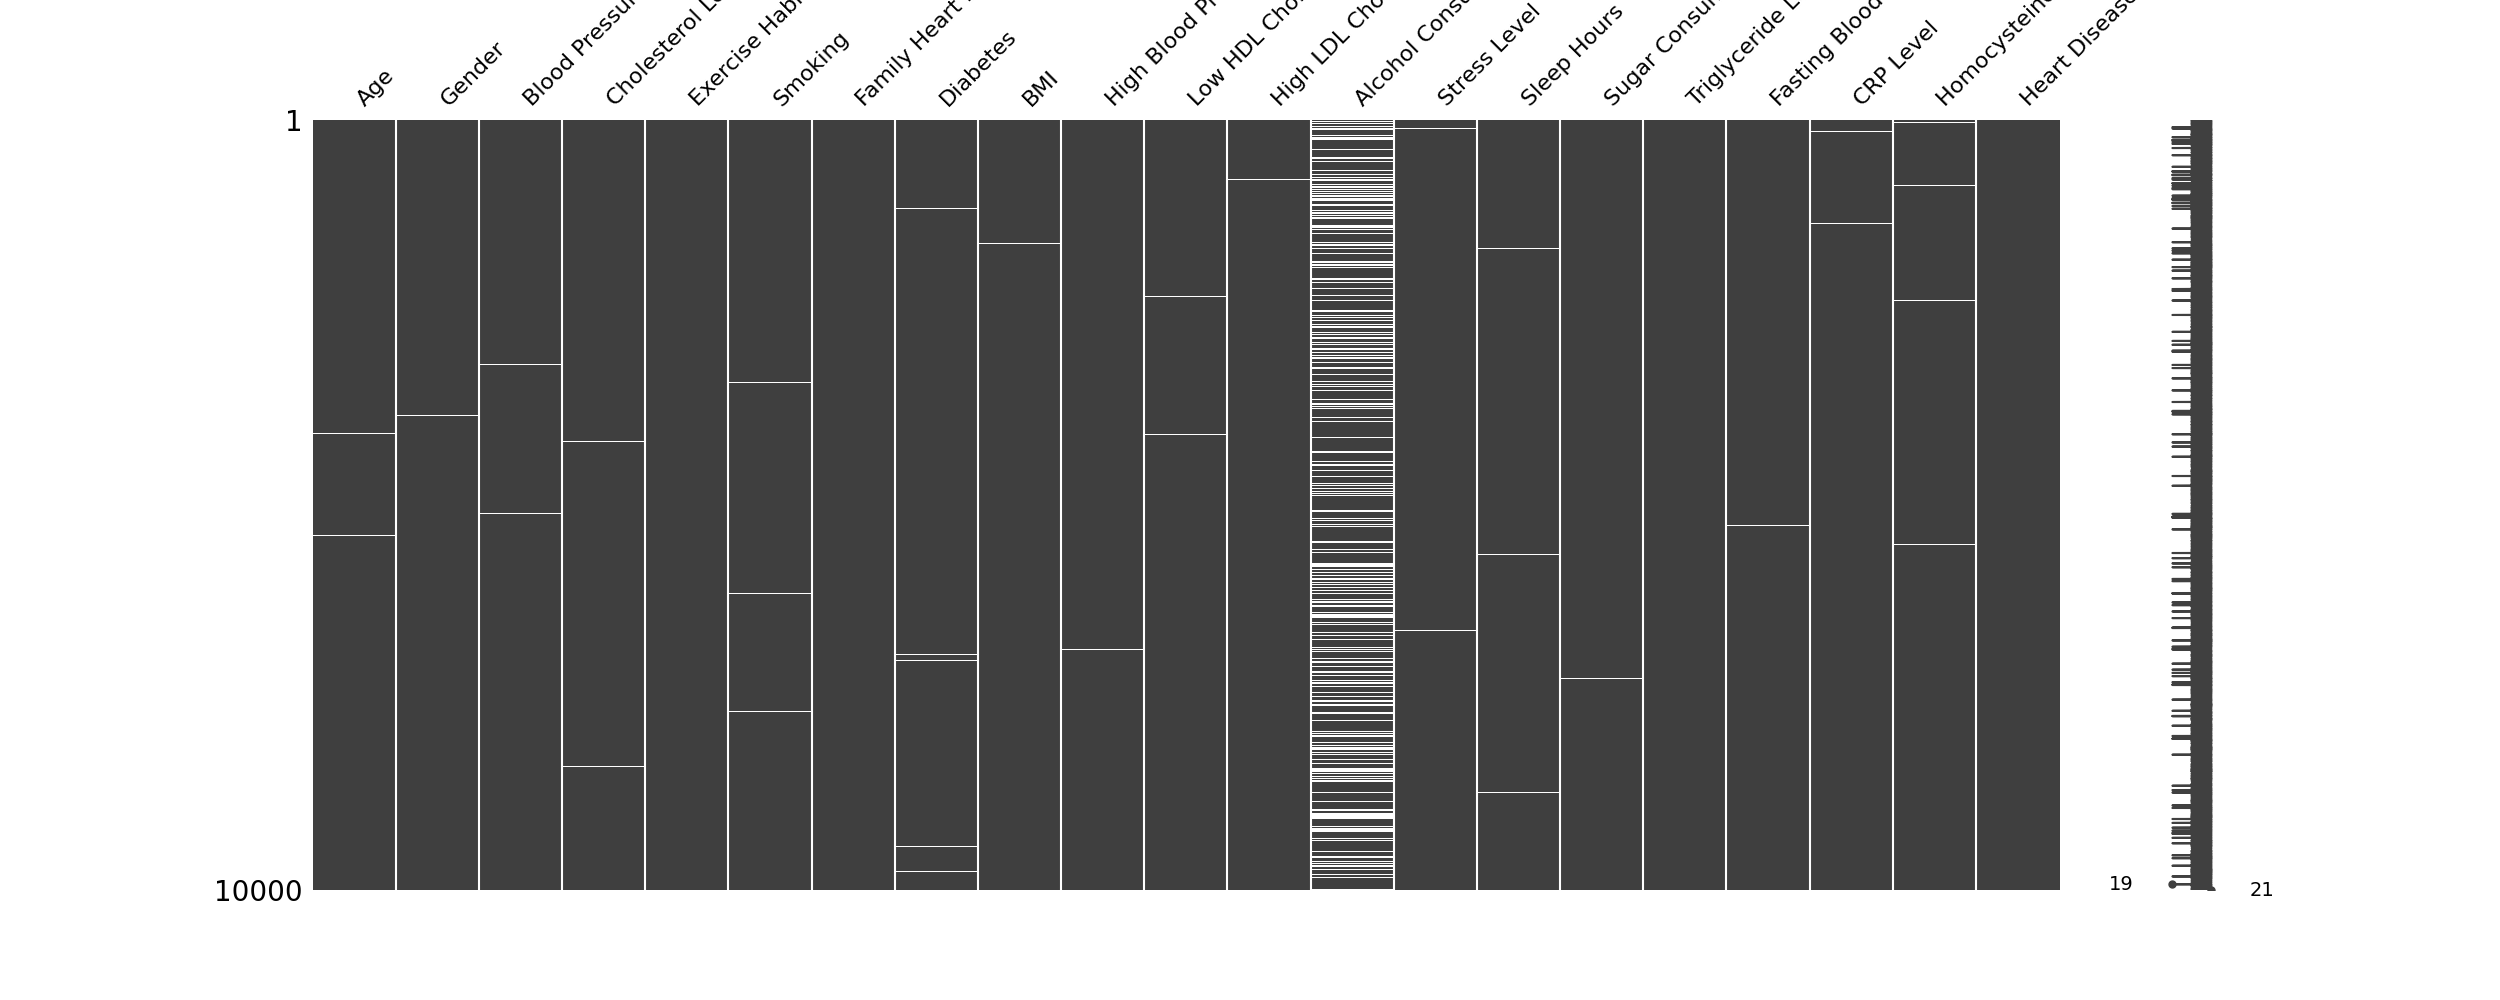
\includegraphics[width=0.8\textwidth]{./pictures/missing_values_matrix.png}
    \caption{Missing Values Matrix Visualization}
\end{figure}

% \begin{figure}[H]
%     \centering
%     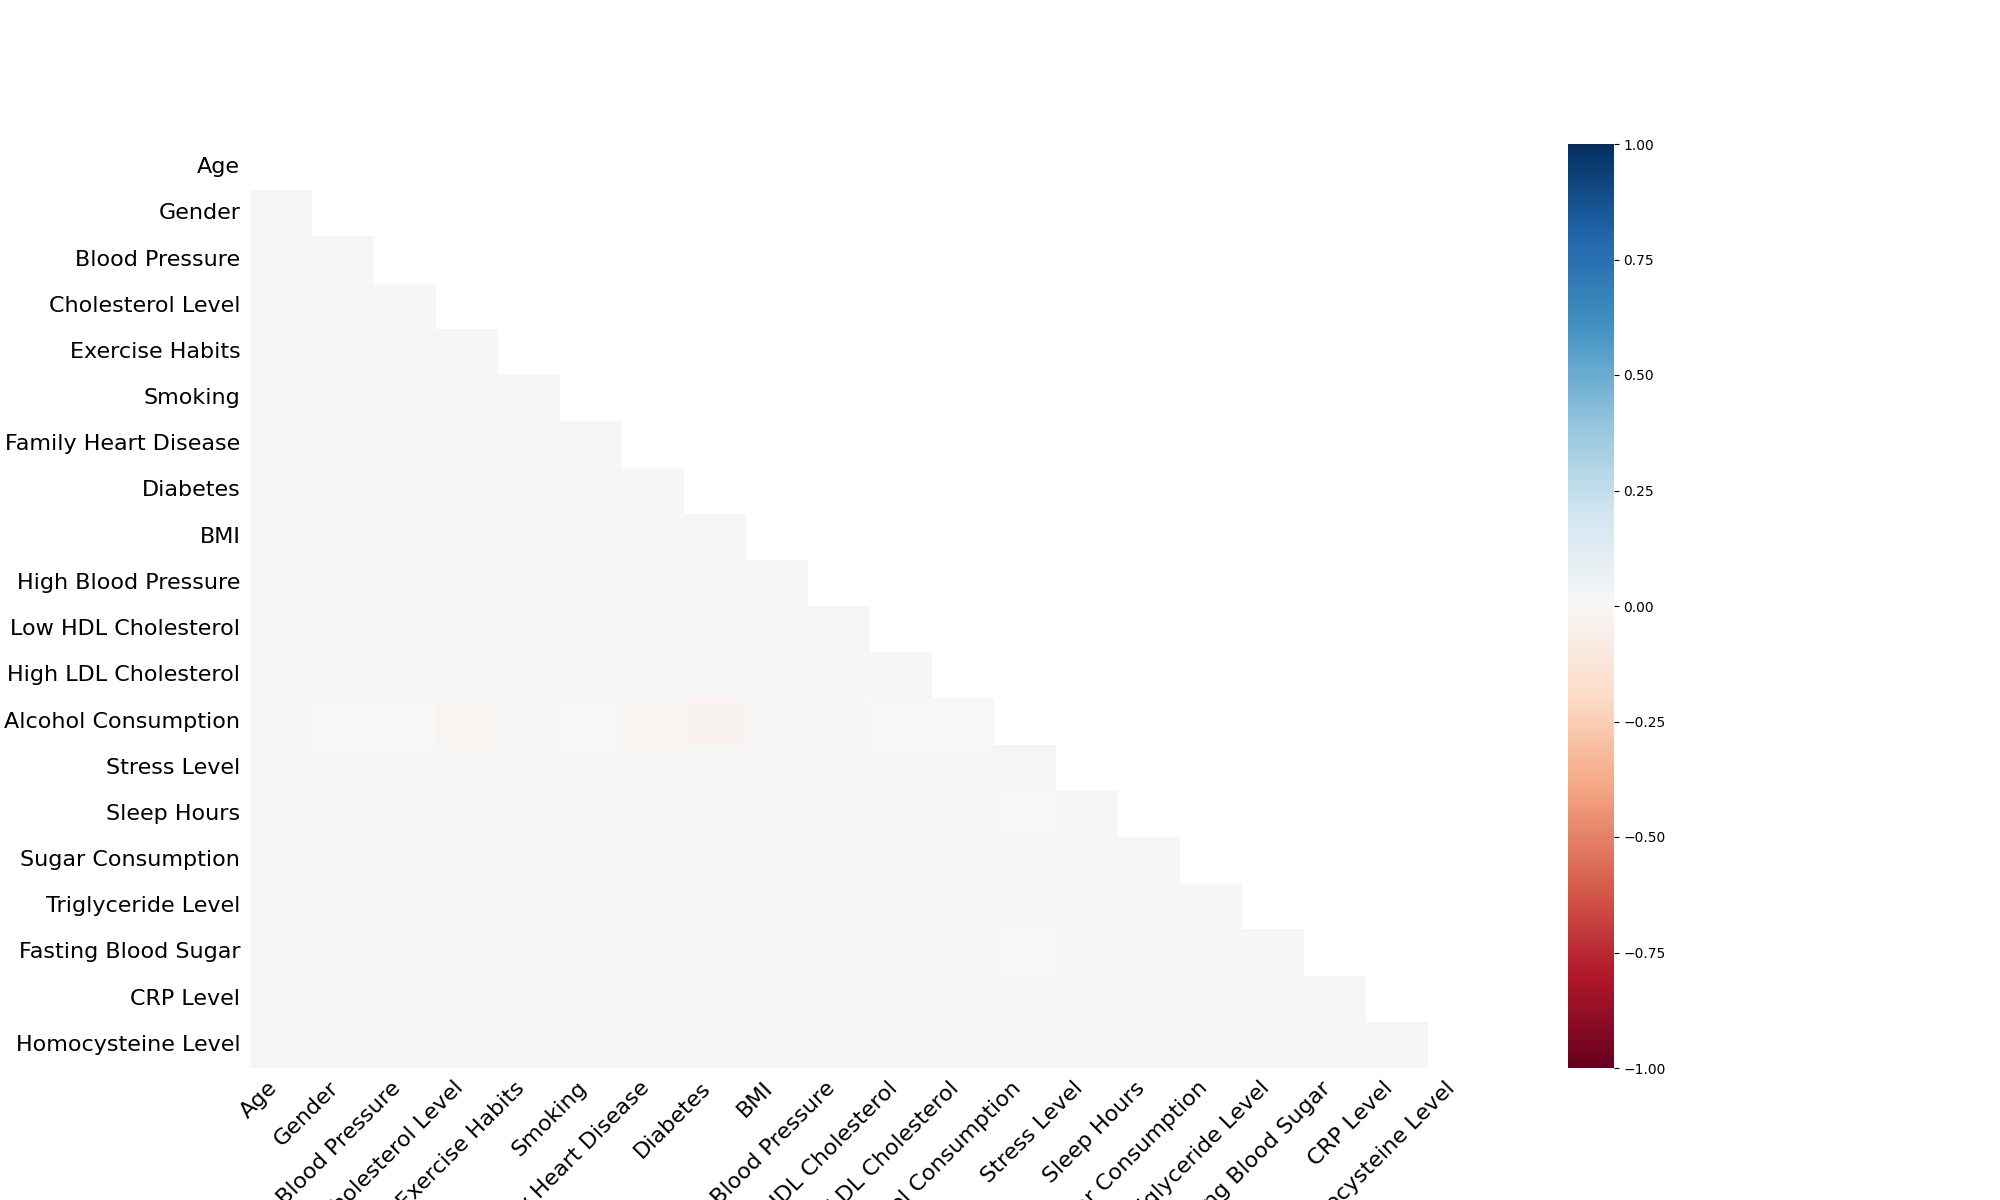
\includegraphics[width=0.8\textwidth]{./pictures/missing_values_heatmap.png}
%     \caption{Missing Values Heatmap Visualization}
% \end{figure}

We able to identify missing data patterns through the matrix above.

\begin{figure}[H]
    \centering
    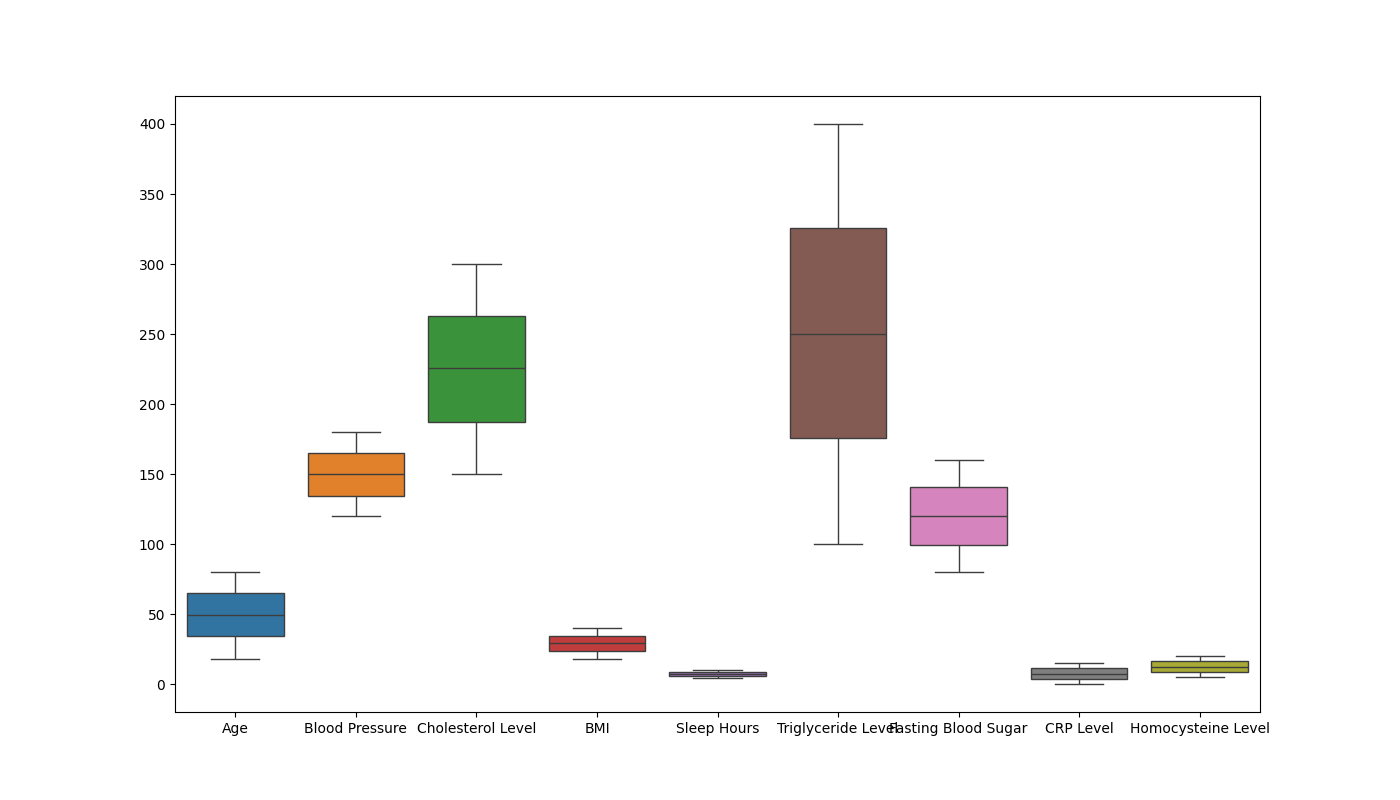
\includegraphics[width=0.8\textwidth]{./pictures/outliers.png}
    \caption{Boxplot Analysis for Outlier Detection}
\end{figure}

Next, we performed outlier analysis using boxplots.
The analysis showed no significant outliers in
the numerical features that would require special treatment.
This allowed us to proceed with the preprocessing without additional outlier handling steps.

To summarize, our preprocessing approach for missing values involved these steps:

\vspace{-0.25cm}
\begin{itemize}
    \vspace{-0.25cm}
    \item \textbf{Feature removal}: We completely removed the 'Alcohol Consumption' feature due to excessive missing data (25.9\%).
          \vspace{-0.25cm}
    \item \textbf{Numerical imputation}: For numerical features, we replaced missing values with column means (affecting 19-30 entries per column).
          \vspace{-0.25cm}
    \item \textbf{Categorical imputation}: For categorical features, we replaced missing values with the most frequent value (mode) in each column.
\end{itemize}

\textbf{Results}: After preprocessing, all missing values were successfully handled, creating a complete dataset with 10,000 entries and 20 features (the original 21 minus Alcohol Consumption).

\subsubsection{Feature Encoding and Transformation}
\vspace{-0.25cm}

For effective model training, we applied these transformations:

\vspace{-0.25cm}
\begin{itemize}
    \vspace{-0.25cm}
    \item \textbf{Categorical encoding}: Converted categorical variables to numerical form using one-hot encoding
          \vspace{-0.25cm}
    \item \textbf{Feature scaling}: Standardized numerical features to have zero mean and unit variance
          \vspace{-0.25cm}
    \item \textbf{Data type conversion}: Optimized data types (e.g., converted Gender to category type)
\end{itemize}
\vspace{-0.25cm}
\textbf{Results}: These transformations produced a machine learning-ready dataset with properly scaled numerical features and encoded categorical variables, enabling efficient model training.

\subsection{Methodological Challenges}

\subsubsection{Feature Selection}
\vspace{-0.25cm}
Determining the most predictive features for heart failure risk
presented a significant challenge. Through visualizations and statistical analysis, we identified several key predictors:

\begin{figure}[H]
    \centering
    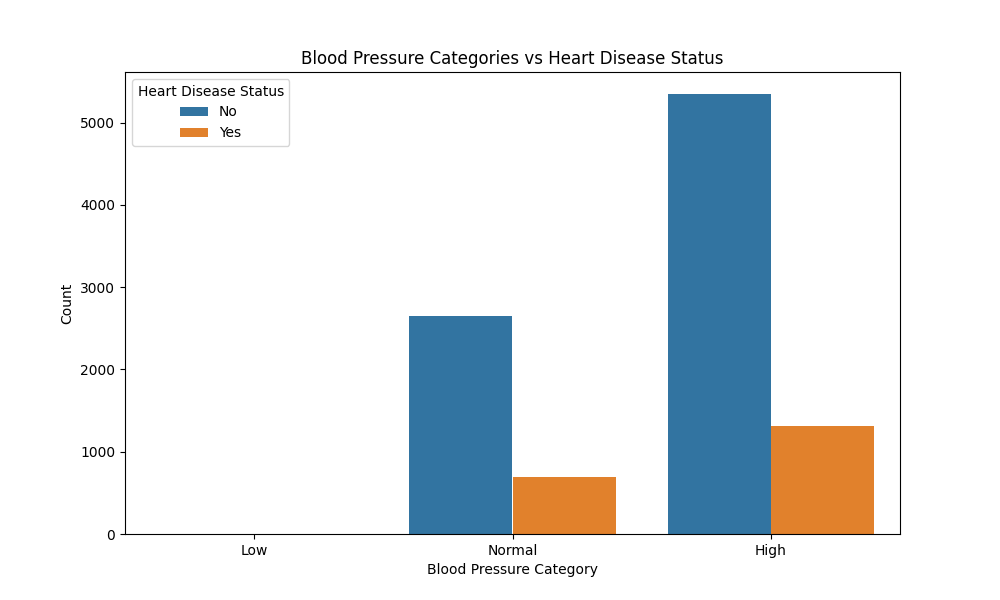
\includegraphics[width=0.8\textwidth]{./pictures/blood_pressure_categories_vs_heart_disease_status.png}
    \caption{Blood Pressure Categories vs Heart Disease Status}
\end{figure}

\textbf{Blood Pressure}: Analysis shows that individuals with higher blood pressure tend to have a higher incidence of heart disease.

\begin{figure}[H]
    \centering
    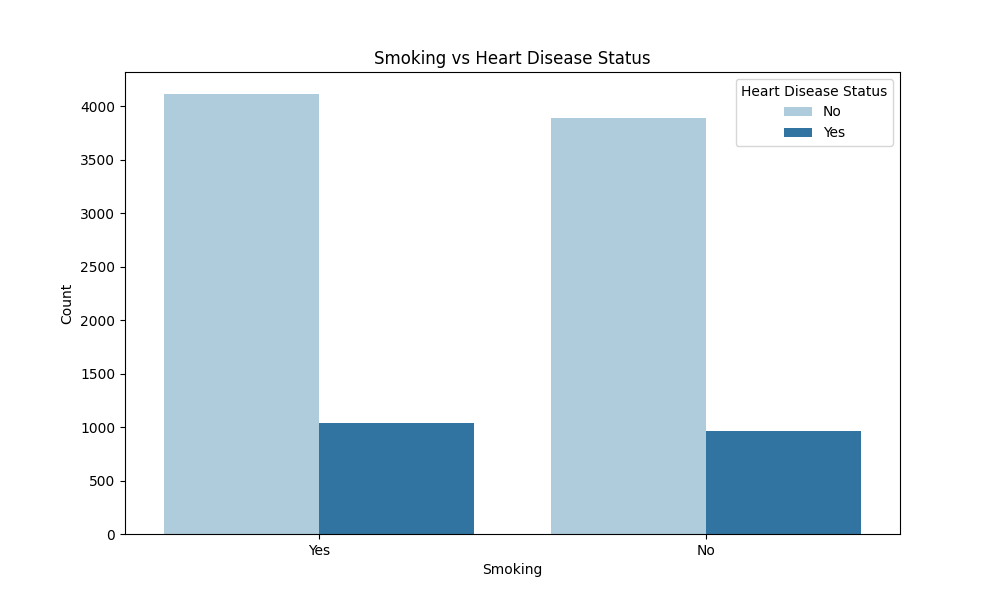
\includegraphics[width=0.8\textwidth]{./pictures/smoking_vs_heart_disease_status.png}
    \caption{Smoking vs Heart Disease Status}
\end{figure}

\textbf{Smoking}: The visualization above reveals a clear relationship between smoking habits and heart disease status.

Our initial approach included using ANOVA
F-tests to identify statistically significant features, but the
effectiveness of this method varied across different subsets
of our data.
The interrelationships between various health indicators complicated the feature
selection process, as some features that appeared
individually insignificant could become important when
considered in combination with others.

\subsubsection{Model Selection and Optimization}
\vspace{-0.25cm}
Selecting the most appropriate machine learning models for heart failure prediction required balancing accuracy, interpretability, and computational efficiency. Our project implements Neural Network and Support Vector Machine models, each presenting unique challenges:

\begin{itemize}
    \vspace{-0.25cm}
    \item \textbf{\greencheck \space Neural Network (NN)}: Our deep learning approach required careful architecture design, including determining the optimal number of hidden layers, neurons per layer, and activation functions. Additionally, preventing overfitting through techniques like dropout and early stopping required extensive experimentation.

    \item \textbf{\greencheck \space Decision Tree Classifier}: While effective for high-dimensional classification, optimizing SVM required extensive hyperparameter tuning, particularly for the regularization parameter (C) and kernel selection (linear, polynomial, RBF). Finding the right balance between model complexity and generalization capability was challenging.
\end{itemize}

\subsection{Implementation Challenges}
\begin{itemize}
    \item \textbf{Neural Network (NN)} - During development, our neural network model encountered a very common issue, overfitting. The initial implementation would have 94\% accuracy on average with the training data, and 70\% accuracy on average with the testing data. To battle this overfitting issue, a dropout layer and regularization was implemented.
    \item \textbf{Support Vector Machine (SVM)} - Implementing this model came with its difficulties due to the nature of the dataset used. The dataset is heavily biased towards no disease which caused performance to initially seem high (80\%) although this was not acutally the case. Cross validation did reveal that this was an issue and to resolve it,  balanced class weight was used to help with the bias.
\end{itemize}

% \subsubsection{Data Integration}
% \vspace{-0.25cm}
% Our project utilized a single comprehensive dataset (Heart Disease UCI),
% eliminating integration challenges that would exist with multiple data sources.
% This approach allowed us to focus on model development rather than data harmonization tasks,
% ensuring consistency in feature definitions and measurement units throughout the analysis.

\subsubsection{Cross-Validation Strategy}
\vspace{-0.25cm}
To ensure robust model evaluation and prevent overfitting,
we implemented \textbf{k-fold cross-validation} + \textbf{bootstraping} with \textbf{k} values ranging from 5 to 20.
This standardized approach was consistently applied across all models to facilitate
fair comparison of performance metrics.
% The cross-validation process helped us validate our models' generalizability by testing them on multiple different training and validation splits of the data.

% TODO: add the implementation of the models here
\section{Models Implemented}
The project implements the following machine learning models for heart
failure risk prediction:
\begin{itemize}
    \vspace{-0.25cm}
    \item \textbf{Neural Network (NN)}: A feed-forward multilayer perceptron trained on the UCI dataset with early stopping and dropout regularization.
    \item \textbf{Decision Tree Classifier}: A decision tree classifier wrapped in an \texttt{imblearn} pipeline
    \item \textbf{Support Vector Machine (SVM)}: A kernel-based classifier using radial basis function (RBF) kernel with balanced class weights to address the dataset imbalance. The model attempts to find an optimal hyperplane that maximizes the margin between heart disease and non-heart disease cases in a transformed feature space.
\end{itemize}


% \begin{tcolorbox}[infobox={Insights and Solutions}]
%     Despite these challenges, our team implemented several effective solutions:
%     \vspace{-0.25cm}
%     \begin{itemize}
%         \item a
%         \item a
%         \item a
%         \item a
%     \end{itemize}
% \end{tcolorbox}

\section{Each Member's Implementation and Evaluation}

\subsection{Member 1 (Marcos Villanueva Abreu, undergraduate)}

\begin{tcolorbox}[
        title=Neural Network Implementation,
        colback=lightblue!30,
        colframe=darkblue,
        boxrule=0.5pt,
        fonttitle=\bfseries\sffamily\footnotesize,
        fontupper=\footnotesize
    ]
    \textbf{Model and Implementation details:}

    The Neural Network model was implemented with the following key components:
    \begin{itemize}[leftmargin=*, itemsep=2pt, parsep=0pt]
        \item Two hidden layers, and one dropout layer that sets 5\% of the inputs to 0.
        \item Each hidden layer has 512 nodes and used ReLU as their activation function.
        \item Output layer has 2 nodes (binary classification).
        \item Hidden layers use L1 and L2 regularization to reduce overfitting.
        \item Data is standardized, nominal values are one hot encoded and ordinal values are encoded with an ordinal encoder.
        \item Input layer has 26 nodes (7 additional nodes from the 19 features due to the encoding).
    \end{itemize}

    \textbf{Evaluation Results:}
    \begin{itemize}[leftmargin=*, itemsep=2pt, parsep=0pt]
        \item Accuracy: 80.43\%
        \item Precision: 80.43\%
        \item Recall: 80.43\%
        \item F1 Score: 89.15\%
        \item AUC-ROC: 80.43\%
    \end{itemize}
\end{tcolorbox}

\subsection{Member 2 (Van Ky Thien Nguyen, graduate)}

\begin{tcolorbox}[%
        title=Decision Tree Classifier Implementation,
        colback=lightpurple!30,
        colframe=mediumpurple,
        boxrule=0.5pt,
        fonttitle=\bfseries\sffamily\footnotesize,
        fontupper=\footnotesize
    ]
    \textbf{Model and implementation details:}
    \begin{itemize}[leftmargin=*, itemsep=2pt, parsep=0pt]
        \item Decision-tree classifier wrapped in an \texttt{imblearn} pipeline
        \item Grid-search hyper-tuning for \verb|max_depth| $\in\{3,5,7,\text{None}\}$ and \verb|min_samples_leaf| $\in\{1,5,10\}$
        \item SMOTE oversampling to combat class imbalance
        \item One-hot encoding for any nominal categorical features (none in this run)
        \item Stratified $k$-fold cross-validation with $k\in\{5,\dots,20\}$, executed sequentially (\verb|n_jobs=1|)
    \end{itemize}

    \textbf{Evaluation results ($k$-fold, $k=5\text{–}20$):}
    \begin{itemize}[leftmargin=*, itemsep=2pt, parsep=0pt]
        \item Accuracy: \textbf{65.9 \% – 73.3 \%}
        \item Precision: \textbf{6.9 \% – 15.1 \%}
        \item Recall: \textbf{11.8 \% – 25.8 \%}
        \item F\textsubscript{1} score: \textbf{8.7 \% – 19.0 \%}
        \item AUC-ROC: \textbf{50.2 \% – 51.9 \%}
    \end{itemize}

    \textbf{Train-on-full dataset snapshot:}
    \begin{itemize}[leftmargin=*, itemsep=2pt, parsep=0pt]
        \item Accuracy: 60.5 \%
        \item Precision: 21.4 \%
        \item Recall: 36.5 \%
        \item F\textsubscript{1} score: 27.0 \%
        \item AUC-ROC: 52.2 \%
    \end{itemize}
\end{tcolorbox}

%-------------------------------------------------
\subsection{Member 3 (Kaitlin Chan, undergraduate)}
%-------------------------------------------------
\begin{tcolorbox}[%
        title=K-Nearest Neighbors Classification,
        colback=lightgreen!30,
        colframe=darkgreen,
        boxrule=0.5pt,
        fonttitle=\bfseries\sffamily\footnotesize,
        fontupper=\footnotesize
    ]
    \textbf{Implementation details:}
    \begin{itemize}[leftmargin=*, itemsep=2pt, parsep=0pt]
        \item Encoded binary categorical variables (\textit{Yes/No}, \textit{Female/Male}) to  \numrange{0}{1}
        \item Mapped ordinal features (\textit{Low/Medium/High}) to integer scores \numrange{0}{2}
        \item Standardized all predictors with \texttt{StandardScaler}
        \item Tuned $k$ from 1\,–\,10 on a 20 \% hold-out set; selected $k\!=\!5$ for reporting
        \item Assessed model stability via stratified $k$-fold CV ($k\!=\!5\text{–}20$)
    \end{itemize}

    \textbf{Evaluation Results (hold-out, $k=5$):}
    \begin{itemize}[leftmargin=*, itemsep=2pt, parsep=0pt]
        \item Accuracy: \textbf{77.0 \%}
        \item Precision: \textbf{24.8 \%}
        \item Recall: \textbf{7.2 \%}
        \item F1 Score: \textbf{11.2 \%}
        \item AUC-ROC: \textbf{51.3 \%}
    \end{itemize}
\end{tcolorbox}


\subsection{Member 4 (Austin Choi, undergraduate)}

\begin{tcolorbox}[
        title=Visualization and Model Evaluation,
        colback=mediumblue!30,
        colframe=darkblue,
        boxrule=0.5pt,
        fonttitle=\bfseries\sffamily\footnotesize,
        fontupper=\footnotesize
    ]
    \textbf{Implementation details:}
    \begin{itemize}[leftmargin=*, itemsep=2pt, parsep=0pt]
        \item Encoded binary categorical variables (\textit{Yes/No}, \textit{Female/Male}) to  \numrange{0}{1}
        \item Mapped ordinal features (\textit{Low/Medium/High}) to integer scores \numrange{0}{2}
        \item Standardized all predictors with \texttt{StandardScaler}
        \item Set class weight to balanced to account for imbalanced data
        \item Applied RBF kernel trick to help improve accuracy
        \item Assessed model stability via stratified $k$-fold CV ($k\!=\!5\text{–}20$)
    \end{itemize}

    \textbf{Evaluation Results:}
    \begin{itemize}[leftmargin=*, itemsep=2pt, parsep=0pt]
        \item Accuracy:55.25%
        \item Precision: 68%
        \item Recall: 55%
        \item F1 Score: 60%
        \item AUC-ROC: 48.70
    \end{itemize}
\end{tcolorbox}

\section{Discussion}
\begin{itemize}
    \item \textbf{Neural Network (NN)} – As we can observe above from the evaluation
          results of the model, the accuracy, recall,
          and precision are the same values while the AUC is very similar
          (the last couple of decimal points are different) to the values
          of the aforementioned metrics. This
          could be that the model is predicting the samples correctly, meaning
          there are no false positives or false negatives. This
          scenario is rare, so our team will need to investigate further to improve performance.
          Another observation is that training and testing accuracies often match when validating with \(k\)-fold;
          individual folds differ, but the overall averages tend to coincide.
    \item \textbf{Decision Tree Classifier} – While cross-validated accuracy is respectable
          $\,\approx$\,\textbf{66--73\%},
          the model’s precision and recall remain low ($\approx$\,\textbf{7--26\%}), and its AUC stays just above random chance
          ($\approx$\,\textbf{50--52\%}). These figures indicate the tree still struggles to isolate positive cases despite oversampling and tuning. Future work should investigate richer feature engineering, ensemble variants (e.g., balanced random forests, gradient boosting), or cost-sensitive learning to lift minority-class detection without sacrificing overall stability.
    \item \textbf{K-Nearest Neighbors (KNN)} – Although overall accuracy is high ($\approx 77\%$), the model captures very few positive cases (recall $\approx 7\%$) and its AUC hovers near random chance ($\approx 51\%$). This suggests a strong bias toward the majority class. Distance-weighted voting, alternative distance metrics, or combining KNN with resampling/ensemble strategies could help boost minority-class detection.
    \item \textbf{Support Vector Machine (SVM)} – We can see that performance for SVM is lower than those of the other models even after various precprocessing techniques and kernel trick were applied. The model's accuracy ($\approx 55\%$) is only slightly better than random guessing wile its AUC is right below random ($\approx 48\%$). This perfomance can be seen across all K-fold validations ($\approx 54\%$). This performance is due toe the class imbalance since the dataset heavily leans towards no heart disease. This can be seen when class weight is not set to balanced since the model will predict 0 every time.
\end{itemize}



\end{document}
